

\section{Further outreach information}
\label{sec:outreach}
As mentioned in Section~\ref{sec:seleff}, we want to provide 
enough information so that anybody can use their favorite Monte Carlo
generator of new physics, define an acceptance at the hard 
scatter level (status = 3 in Pythia), and correctly estimate
the efficiency for this new physics model to within 50\% or so.

The relevant information on selection efficiencies is 
given in Section~\ref{sec:seleff}.  In this Section we give the 
second missing ingredients for this program, namely the 
95\% upper limits on the number of events for the various 
signal regions.  We also show how well our efficiency model 
works in a few cases.

\subsection{Limits on number of events}
\label{sec:outreachlimits}
In Table~\ref{tab:outreach} we summarize the 
results of the counting experiments in the various signal 
regions that are given in more 
details in Tables~\ref{tab:yield_baseline} 
to~\ref{tab:yield_ht200met503btag}; in addition, for each signal 
region we give the 95\% CL upper limit on the number of 
non-SM events ($N_{UL}$) calculated using the $CL_s$ method.

The value of $N_{UL}$ is a key ingredient to allow phenomenologists
to interpret our data: basically any model that predicts an 
event yield $> N_{UL}$ is excluded at 95\% CL.  Uncertainties 
in the efficiency need to be included in $N_{UL}$.  This is tricky 
because the components of the efficiency uncertainty associated 
with the JES and the btagging differ model-by-model.  Fortunately,
this is not a big effect.  In order to show that it is not, in 
Table~\ref{tab:outreach} we give $N_{UL}$ with uncertainties of 
12\%, 20\%, and 30\%. The first value (12\%) corresponds to the 
``minimum uncertainty'', {\em i.e.} the uncertainty due to 
lepton efficiency and luminosity only; the other two values (20\%
and 30\%) are ``typical'' uncertainty values when including
JES and btagging.

\begin{table}
\begin{tabular}{|l|c|c|c|c|c|c|c|}
\hline
 & Region 1 &  Region 2 & Region 3 & Region 4 & Region 5 & Region 6 & Region 7\\
\hline
No. of jets & $\geq 2$ &  $\geq 2$ &  $\geq 2$ &  $\geq 2$ &  $\geq 2$ &  $\geq 2$ &  $\geq 3$ \\
No. of btags & $\geq 2$ &  $\geq 2$ &  $\geq 2$ &  $\geq 2$ &  $\geq 2$ &  $\geq 2$ &  $\geq 3$ \\
Lepton charges & $++/--$ & $++$ & $++/--$ & $++/--$ & $++/--$ & $++/--$ & $++/--$ \\
\met & $\geq 30$ GeV & $\geq 30$ GeV & $\geq 120$ GeV & $\geq 50$ GeV & $\geq 50$ GeV & $\geq 120$ GeV & $\geq 50$ GeV \\
$H_T$ & $\geq 80$ GeV & $\geq 80$ GeV & $\geq 200$ GeV & $\geq 200$ GeV & $\geq 320$ GeV & $\geq 320$ GeV & $\geq 200$ GeV \\
\hline
BG from charge flips & $1.1 \pm 0.2$ & $0.5 \pm 0.1$ & $0.05 \pm 0.01$ & $0.3 \pm 0.1$ & $0.12 \pm 0.03$ & $0.026 \pm 0.009$ & $0.008 \pm 0.004$ \\ 
BG from fakes & $3.4 \pm 2.0$ &  $1.8 \pm 1.2$ &  $0.32 \pm 0.50$ &  $1.5 \pm 1.1$ &  $0.81 \pm 0.78$ &  $0.15 \pm 0.45$ &  $0.15 \pm 0.45$ \\
BG from rare SM & $3.2 \pm 1.6$ & $2.1 \pm 1.1$ & $0.56 \pm 0.28$ & $2.0 \pm 1.0$ & $1.04 \pm 0.52$ & $0.39 \pm 0.20$ & $0.11 \pm 0.06$ \\
\hline
Total expected BG  & $7.7 \pm 2.6$ & $4.4 \pm 1.6$ & $0.9 \pm 0.6$ & $3.7 \pm 1.5$ & $2.0 \pm 0.9$ & $0.6 \pm 0.5$ & $0.3 \pm 0.5$ \\
No. data events & 7 & 5 & 2 & 5 & 2 & 0 & 0 \\
\hline
$N_{UL}$ (12\% uncert.) & 7.4 & 6.9 & 5.2 & 7.3 & 4.7 & 2.8 & 2.8 \\
$N_{UL}$ (20\% uncert.) & 7.7 & 7.2 & 5.4 & 7.6 & 4.8 & 2.8 & 2.8 \\
$N_{UL}$ (30\% uncert.) & 8.1 & 7.6 & 5.8 & 8.2 & 5.1 & 2.8 & 2.8 \\
\hline
\end{tabular}
\caption{\label{tab:outreach} A summary of the results of this search.  For each signal region,
we show its most important kinematical requirements, the prediction for the three background 
(BG) components as well as the total, the event yield, and the 95\% CL upper 
limit on the number of non-SM events in each region calculated under three different 
assumptions for the event efficiency uncertainty (see text for more details).}
\end{table}


\subsection{Testing the efficiency model}
\label{sec:outreachtest}

The efficiency model is evaluated by applying it to a few scenarios considered in Section~\ref{sec:stampCollecting}.  For each model considered here, points near the exclusion curve are selected and the yield obtained by applying the full analysis selection is compared to that estimated by applying the efficiencies detailed in Section~\ref{sec:seleff} to generator level objects.  Figure~\ref{fig:zprimeefftest} shows the performance of the efficiency model applied to the scenario of same sign top production due to t-channel exchange of a new massive $Z'$ boson.  The comparison was performed using the same signal region considered in Section~\ref{sec:sstops}.  The estimated and actual yields agree to within 20\%.  When the mass of the $Z'$ is large compared to the mass to the top, the mass of the boson only weakly influences the kinematics of the final state so that the performance of the efficiency model is expected to be relatively constant, as observed.

\begin{figure}[htb]
\begin{center}
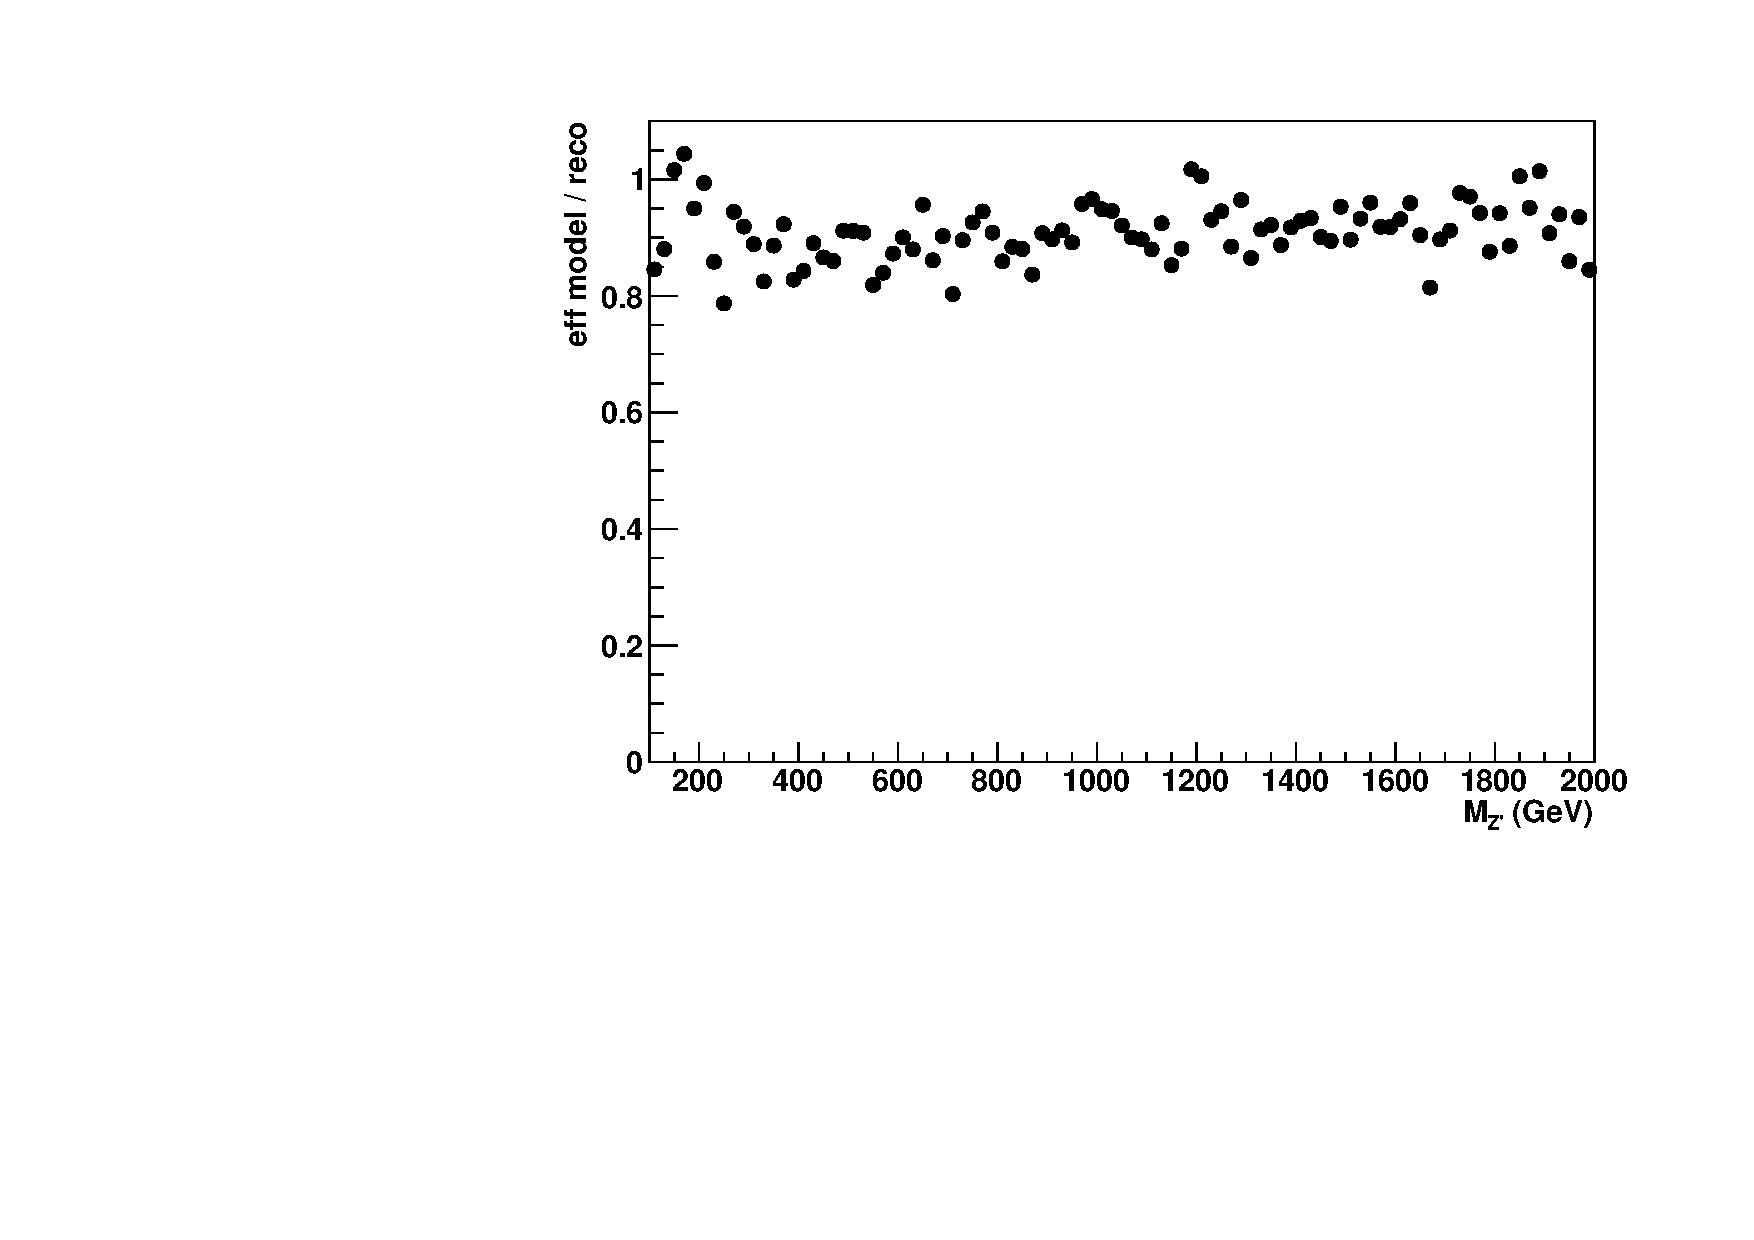
\includegraphics[width=0.95\linewidth]{figs/zprime_eff_test.pdf}
\caption{Test of the efficiency model applied to same sign top production due to a $Z'$.  The figure shows the ratio of the yield estimated by applying the efficiency model to generator level objects to the yield obtained by applying the full analysis selection to reconstructed objects.  Estimated and actual yields agree to within 20\%.
\label{fig:zprimeefftest}}
\end{center}
\end{figure}

Several models involving stop or sbottom production were also considered in Section~\ref{sec:stampCollecting}.  As a worst case scenario, the efficiency model was tested for a few relevant points in the parameter phase space for the $\widetilde{g}$ to $t\widetilde{t}$ model.  The results of these tests are recorded in Table~\ref{tab:gluinostopefftest} .  The comparison was performed using the $\Ht > 320$ GeV, $\met > 120$ GeV signal region.  Estimated yields are found to agree with those obtained using the full analysis selection to within 50\%.

\begin{table}
\begin{center}
\begin{tabular}{c | c c c}
\hline\hline
$m(\widetilde{g}), m(\widetilde{t})$ (GeV) & Actual Yield &  Estimated Yield & Estimated / Actual \\
\hline
800, 280 & 133 & 181 & 1.36 \\
800, 430 & 125 & 184 & 1.47 \\
650, 380 & 99 & 146 & 1.48 \\
\hline\hline
\end{tabular}
\caption{\label{tab:gluinostopefftest} Test of the efficiency model applied to the $\widetilde{g}$ to $t\widetilde{t}$ model.  The table shows the ratio of the yield estimated by applying the efficiency model to generator level objects to the yield obtained by applying the full analysis selection to reconstructed objects.  Estimated and actual yields agree to within 50\%}
\end{center}
\end{table}